\section{Task 1 Forward Kinematics}
\subsection{Task 1.1}
%\subsection{Task 1.1 original Denavit-Hartenberg convention}
\label{title:Task1.1}

%define open-chain

\textbf{Task 1.1: Present the forward kinematics computations for an open-chain manipulator with n joints using the original Denavit-Hartenberg (DH) convention. See, e.g., Chapter 2 in the robotics book by Siciliano et al.}

Denavit-Hartenberg (DH) convention is used to describe the position of joints and links. The DH convention is a minimal line representation, meaning that it is uses 4 parameters to describe the 3D space and the 6 degrees of freedom (DOF) motion the robot is working in. DH parameters also can only describe translation for prismatic joints and rotation for revolute joints. However in many applications of robotics the other joints such as the helical and ball-and-socket joint can be broken down to revolute and prismatic joints if only one axis is analyzed at a time. An open-chain in kinematics is where there is series of joints and links connected to one another, and only one of the joints is connected to the ground, whilst in a closed chain both end of a series of links and joints are connected to the ground. See figure \ref{fig:openvsclosed} for a visual explanation.

\begin{figure} [H]
    \centering
    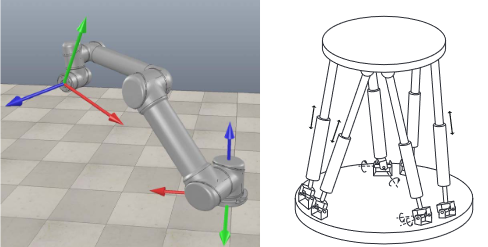
\includegraphics{Images/Task1.1&1.2/openvsclosed.png}
    \caption{The left robotic arm is a open chain system, whilst the Stewart-Gough platform to the right is closed chain system}
    \label{fig:openvsclosed}
\end{figure}

The figure \ref{fig:openvsclosed} clearly shows that the series of links and joints are fixed in only one end of the arm in the picture to the left, whilst in the picture to the right (the Stewart-Gough platform), all links and joints are fixed on both ends. On the platform on the top and to the platform on the bottom.

A prismatic joint is a joint that moves in a singular and linear direction, and it's motion is a extension or retraction displacement. This means that it only has 1 degree of freedom. As is shown in figure \ref{fig:prismatic-revolute}

A revolute joint also has 1 degree of freedom, and it rotates about one axis, and is much like a point on cylinder, that is rotating about its z-axis. As is shown in figure \ref{fig:prismatic-revolute}

\begin{figure} [H]
    \centering
    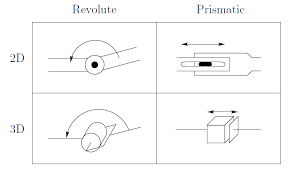
\includegraphics{Images/Task1.1&1.2/prisrevol.png}
    \caption{To the left is a revolute joint showina rotation about one axis, first in 2 dimensions (2D) and then in 3 dimensions (3D). And to the right is prismatic joint showing the translational motion first in 2D and then in 3D}
    \label{fig:prismatic-revolute}
\end{figure}

In this chapter we will present the forward kinematics computations for an open-chain manipulator or end-effector with n joints using the original DH parameters. 

\subsubsection{Denavit-Hartenberg parameters and rules}
For the Denavit-Hartenberg (DH) convention to be used there are 4 rules that need to be true for the it to be possible to create a mathematical reference of the end effector's position according to the reference or base position. In addition we only need as mentioned 4 parameters do define the 6 degrees of freedom (DOF), 3 for rotation and 3 for translation. 

%explain the figure below
\begin{figure}[H]
    \centering
    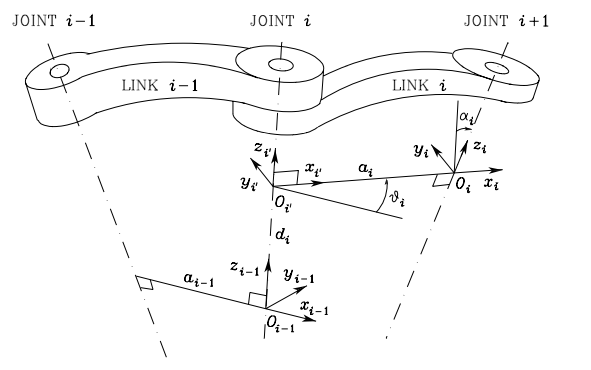
\includegraphics{Images/Task1.1&1.2/DH-original.png}
    \caption{Denavit-Hartenberg kinematic parameters}
    \label{fig:DH-OG}
\end{figure}

Using figure \ref{fig:DH-OG}, the axis \textit{i} stands for the joint axis connecting link \textit{i} - 1 to link \textit{i}. And to use the DH convention for n links in an open chain, the frame \textit{i} is defined using the following rules: 

\begin{itemize}
    \item The \(z_\textit{i}\) axis is coincident and parallel with joint axis \textit{i} + 1, see figure \ref{fig:DH-OG} for reference.
    \item Assure that \textit{O_i} that is at the intersection of axis \textit{z_i} is with a common normal to axes \textit{z_i-1} and \textit{z_i}. And assure that origin \textit{O_i^'} is at the normal with axis \textbf{z_i-1}.
    \item The x axis is parallel with the common normal \(x_n = z_n \times  z_n-1\) with positive direction from joint \textit{i} to joint \textit{i+1}.
    \item The y-axis is chosen following the z and x axis, using the right hand rule.
\end{itemize}
% these rules are paraphrased from siciliano, remember to mention that, there is not a way to rewrite the rules in a different way, only to explain them with your own words.
\source{Siciliano}

%explain a common normal with picture? Needed?
 A common normal is the line that is the minimum distance between two lines. Picture?
%explain the right hand rule or no?
The right hand rule as shown in fig

As mentioned DH convention have only 4 parameters, to represent the 6 DOF, 3 for translation and 3 for rotation. This is possible because the  


allows for this, and this is one of the DH criteria. The criteria are the following:
%Linda: it's perhaps good to add picture
\begin{itemize}
    \item \textbf{(DH1):} The axis X(1) is perpendicular to the base axis Z(0)
    \item \textbf{(DH2):}The axis x1 intersects the axis z0 orthogonally (reference)
    \item \textbf{(DH3):} yn axis is made according to the right hand rule, after the z and x axis is adjusted
    \item \textbf{(DH4):} The origin of joint n, is at xn and zn
\end{itemize}

DH parameters is very commonly used in the industry to manipulate and control an arm movement.
%robotarm movement?


\begin{equation}
    T = R_{z \theta} Trans_{z d} Trans_{x r} R_{x a}
\end{equation}
%Linda you can write theta as a symbol: $\theata$
To create a DH parameter equation, there is a rotation theta that happens around the z axis, then a translation d along z axis, than another translation r along the x axis, and rotation along the x axis, to fit to the robot manipulator.
The four parameters described
\begin{itemize}
    \item d: offset along z0 axis to the common normal
    \item theta: angle about z0, from old x0 to x1
    %don't use the theta to make it more clear for the PoE form?
    \item r: length of a common normal
    \item $\alpha$: angle about the common normal, rotating the old z axis to the new axis.
\end{itemize}

This can be written as 
\begin{equation}
    [T] =
    \begin{bmatrix}
        R_{0_1} &  O_{0_1} \\
        0 & 0
    \end{bmatrix}
\end{equation}



\subsubsection{Procedure}


\subsubsection{Special Cases}
Special cases of DH parameters:
\begin{itemize}
    \item Parallel z axes of the endeffector and reference frame
    \item 
\end{itemize}

%need to only show the math behind it%

